\documentclass{article}
\usepackage{ee105}

%% Makes figure labels bold
\usepackage[labelfont=bf]{caption}

\begin{document}
\thispagestyle{plain}

\tutorial{HP 8116A Function Generator}

\tableofcontents

\section{Introduction}

The HP 8116A is a voltage waveform generator. It can be used to apply periodic voltage waveforms to a circuit (e.g., sinusoids, square waves, triangle waves, and pulses). You will use the function generators to supply time-varying input to circuits for transient or frequency analysis (e.g., to characterize a filter or an amplifier). 

This tutorial starts with quick notes on the most vital information, so if you feel somewhat familiar with the function generator you can check over the quick notes and figure out the details yourself. The later sections include more detailed descriptions of the HP8116A interface.

\section{Quick Notes (to get started fast)}
\begin{itemize}
\item Make sure the ``Disable'' button is off (in the lower-right corner).
\item Set parameters in AMP/OFS mode, not in HIL/LOL mode. If HIL/LOL are lit, push the buttons below HIL/LOL until AMP/OFS are lit.
\item The AMP parameter sets the peak-to-peak amplitude, not the peak amplitude. See Figure \ref{amplitude}.
\item \textbf{Delivered voltage varies with output load impedance.} With an infinite load impedance at the output, the voltage amplitude delivered to the load will be double the panel setting. See Section \ref{voltagedivider}.
\item Choose parameters to adjust with the bottom middle buttons (below the FRQ, WID, etc. LEDs). Change the parameters with the top-right buttons.
\item OFS is voltage offset for the waveform. You can use it to add a constant voltage (DC component) to the wave (e.g. if you want to have a cosine vary around \unit{2}{\volt}).
\item The function generator's ground is \textbf{earth ground}, i.e. the black lead from the BNC cable is not a floating ground. Since the oscilloscope is earth-grounded as well, the function generator and oscilloscope grounds are connected. 
\end{itemize}

\begin{figure}[!htb]
  \centering
  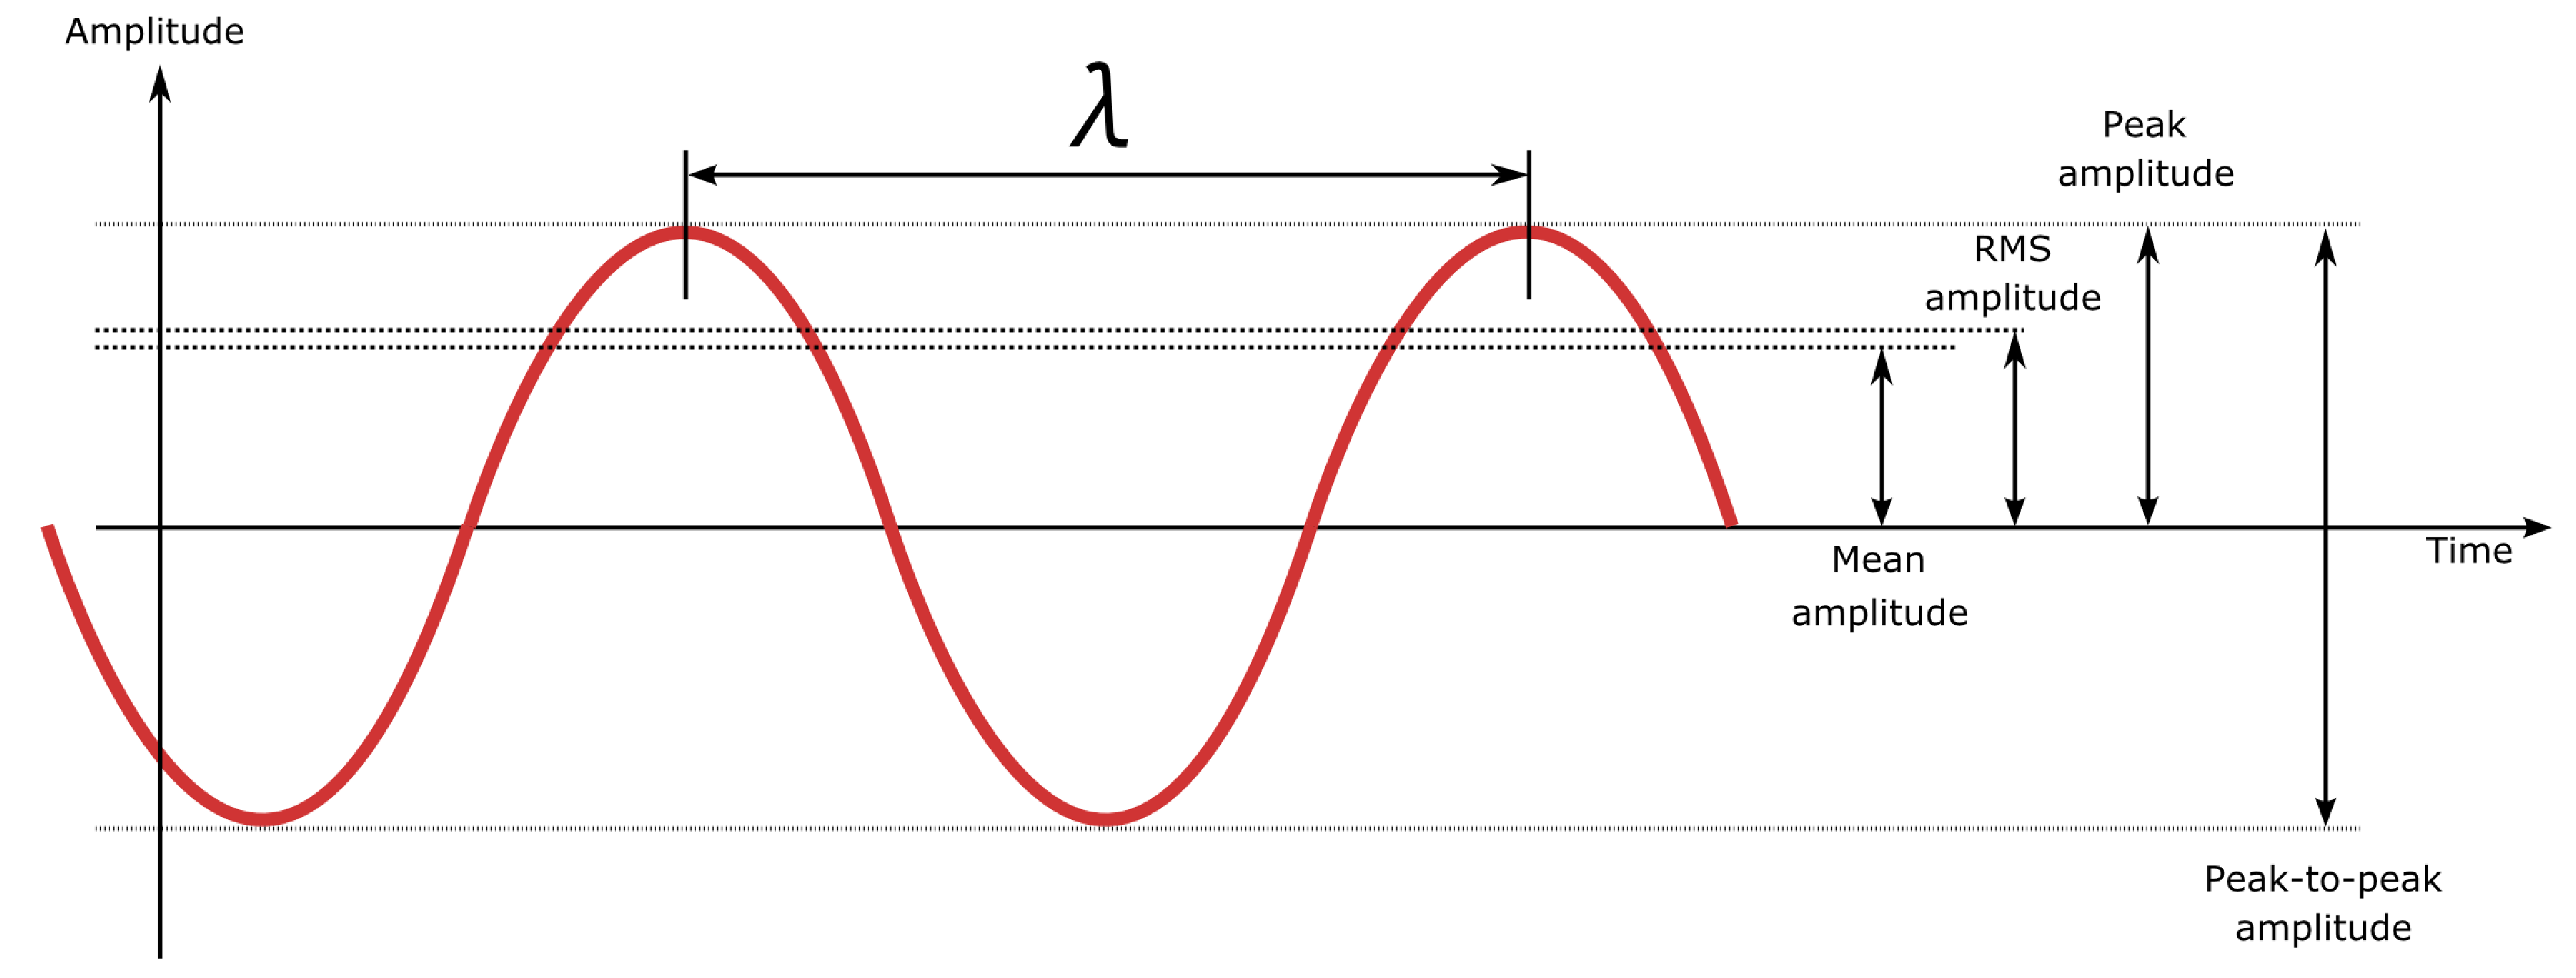
\includegraphics[width=4.0in]{amplitude.eps}
  \caption{Definitions of various wave parameters}
  \label{amplitude}
\end{figure}

\section{Voltage Divider Discussion}
\label{voltagedivider}
When displaying voltage value settings (e.g. the AMP parameter displaying $V_{p-p}$), the function generator panel displays the voltage that will be delivered to the load at the output under the assumption that the total load impedance is \unit{50}{\ohm}. The function generator also has an internal impedance of \unit{50}{\ohm}, and so the load impedance forms a voltage divider with the impedance internal to the function generator. The equivalent voltage divider is shown in Figure \ref{divider}.

\begin{figure}[!htb]
  \input HP8116A_divider
  \centerline{\box\graph}
  \caption{Function generator panel displays voltage values for $R_L=\unit{50}{\ohm}$}
  \label{divider}
\end{figure}

Under the assumption that the load impedance is \unit{50}{\ohm}, the voltage delivered to the load (the effective voltage output) is half the generated voltage of $v_s$. Loading the output with a much greater impedance than \unit{50}{\ohm} (such as connecting the output directly to an oscilloscope) will drop the majority of the voltage across the load, and thus the measured output voltage can be up to double the panel setting. Loading the function generator with $R_L < \unit{50}{\ohm}$ will cause the voltage delivered to be less than the panel setting.

The function generator is often used to create an input signal to amplifiers. Voltage amplifiers often have a high input impedance (e.g. an effectively infinite input impedance for a MOS amplifier), and so the function generator will often be loaded with an infinite $R_L$. Thus the voltage delivered to the amplifier input will often be double the panel setting.

\section{Interface Details}
The power button is in the lower-left corner. The signal output port is in the lower-right corner, and requires a special cable. The trigger output port can be used to send a triggering signal to an oscilloscope, so that the oscilloscope can synchronize its measurement with the signal input (e.g. so as to capture a short pulse).

The notes below correspond to the button groups labeled in Figure 1. They are generally in the order that you would use them to set up a waveform output.

\begin{figure}[!htb]
  \centering
  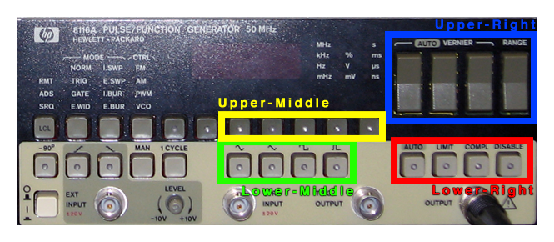
\includegraphics[width=5.0in]{HP8116A.eps}
  \caption{HP 8116A Front Panel}
  \label{HP8116A}
\end{figure}

\subsection{Bottom-Right Buttons}
All of these buttons should be off when you are using the oscilloscope. If any button is lit, you can press it to toggle it off.

The ``Disable'' button disables the voltage waveform output, and it will be on (showing a red light) when the function generator is first turned on. Press it once to turn it off.

\subsection{Bottom-Middle Buttons}
These buttons set the signal shape according to the images on the buttons. There are four options, from left to right:
\begin{itemize}
\item \textbf{Sinusoidal}: A sine or cosine wave. Eigenfunctions of LTI systems.
\item \textbf{Triangle}: Also known as a ``Sawtooth'' wave. 
\item \textbf{Square}: Periodically switches between two values.
\item \textbf{Pulse}: A voltage pulse is sent periodically. The pulse width can be tuned separately from the period (time interval between repeated pulses). The peak value of the pulse can also be set.
\end{itemize}

\subsection{Upper-Middle Buttons}
These four buttons allow you to select a parameter of the wave to adjust with the upper-right buttons (see below for a description of the upper-right buttons). Only one of these parameter buttons is active at once. 

Each button has two labels above it, with only one of the two labels lit at a time. The lit label corresponds to the parameter that is currently selected, and its value will be shown on the display. You will only only need to adjust the FRQ, WID, DTY, AMP, or OFS parameters. If HIL and LOL are lit, press the button beneath LOL until AMP and OFS are lit. 

Here is a list of the parameter labels and their meanings:
\begin{itemize}
\item \textbf{FRQ} Frequency in repetitions/second. In the case of a pulse, this parameter corresponds to the frequency at which repeated pulses are sent. 
\item \textbf{WID} Pulse width
\item \textbf{DTY} Duty cycle, which is defined as the pulse duration and the period of a rectangular waveform.
\item \textbf{AMP} Amplitude, defined as the distance between the base DC voltage and the wave maximum (e.g. height for a pulse).
\item \textbf{OFS} DC voltage offset. The time-varying waveform is offset (``raised'') by the constant offset component (e.g. if you want a sinusoid of amplitude \unit{1}{\volt} centered at \unit{3}{\volt}).
\end{itemize}

For some waveforms, not all above parameters are needed. For example, for a sinusoidal wave, only FRQ, AMP, and OFS might be adjusted.
 
\subsection{Upper-Right Buttons}
Each button resembles a toggle switch, and it can be pushed either ``up'' and ``down'' to adjust values shown on the display. The three buttons on the left adjust the corresponding three digits curerntly on the display (e.g. the leftmost button will adjust the most significant digit on the display). The rightmost will shift between orders of magnitude (e.g. from \milli\volt\ to \volt\ or \milli\hertz\ to \hertz\ to \kilo\hertz\ to \mega\hertz). Pushing a button up once will increment the corresponding digit's value by one, and pushing a button down once will decrement the corresponding digit's value.

\subsection{Display}
The display shows the value of the currently selected parameter. There are points on the right to show the units and order of magnitude (e.g. \milli\volt\ or \volt). The numeric display always shows three digits and a decimal point.

\section{Examples}

\subsection{Sinusoid}
Here are all of the steps necessary to set up a \unit{5}{\kilo\hertz}, \unit{1}{\volt} $V_{p-p}$ sinusoid wave with a \unit{1}{\volt} offset on a large load (much larger than \unit{50}{\ohm}).
\begin{enumerate}
\item Turn on the function generator with the lower-left power button, and enable it by pressing the Disable button in the lower-right (so that the Disable light is off).
\item Press the sinusoid button in the lower-middle set of buttons.
\item Press the FRQ button in the upper-middle set of buttons, and use the upper-right buttons to select \unit{5}{\kilo\hertz} on the display.
\item Pres the AMP button in the upper-middle set of buttons, and use the upper-right buttons to select \unit{500}{\milli\volt} on the display. This step will only produce a \unit{1}{\volt} $V_{p-p}$ wave given a load impedance much larger than \unit{50}{\ohm}. See Section \ref{voltagedivider} for a discussion.
\item Press the OFS button in the upper-middle set of buttons, and use the upper-right buttons to select a \unit{500}{\milli\volt} offset on the display. 
\end{enumerate}

\subsection{Pulse}
Here are all of the steps necessary to set up a \unit{1}{\volt} pulse with \unit{1}{\micro\second} duration and repetition every \unit{10}{\micro\second} on a load impedance much larger than \unit{50}{\ohm}.
\begin{enumerate}
\item Turn on the function generator with the lower-left power button, and enable it by pressing the Disable button in the lower-right (so that the Disable light is off).
\item Press the pulse button in the lower-middle set of buttons (the rightmost button).
\item Press the FRQ button in the upper-middle set of buttons. Since we want \unit{10}{\micro\second} between repetitions, we want $\frac{1}{10\micro} = \unit{10^5}{\hertz}$. Use the upper-right buttons to select \unit{100}{\kilo\hertz}.
\item Press the WID button in the upper-middle set of buttons. Use the upper-right buttons to select a \unit{1}{\micro\second} width.
\item Pres the AMP button in the upper-middle set of buttons, and use the upper-right buttons to select \unit{500}{\milli\volt} on the display. This step will only produce a \unit{1}{\volt} height pulse given a load impedance much larger than \unit{50}{\ohm}. See Section \ref{voltagedivider} for a discussion.
\end{enumerate}

\end{document}